\documentclass[12pt,a4paper,titlepage]{article}
\usepackage[pdftex]{graphicx}
\usepackage[polish]{babel}
\usepackage[utf8]{inputenc}
\usepackage[T1]{fontenc}
\usepackage{tabularx}
\usepackage{tikz}
\usepackage{tikz-qtree}
\usepackage{float}
\usepackage{hyperref}
\usepackage{longtable}
\renewcommand{\labelenumii}{\arabic{enumi}.\arabic{enumii}}
\renewcommand{\labelenumiii}{\arabic{enumi}.\arabic{enumii}.\arabic{enumiii}}
\renewcommand{\labelenumiv}{\arabic{enumi}.\arabic{enumii}.\arabic{enumiii}.\arabic{enumiv}}

\tikzset{every tree node/.style={align=center,anchor=north}}

\title{Prover logiki temporalnej}
\author{Stanisław Maciąg, Piotr Mitana}
\date{2014}



\begin{document}
\newcolumntype{L}[1]{>{\raggedright\arraybackslash}p{#1}}
\newcolumntype{C}[1]{>{\centering\arraybackslash}p{#1}}
\newcolumntype{R}[1]{>{\raggedleft\arraybackslash}p{#1}}

\maketitle

\section{Założenia projektowe}
W ramach projektu zaprojektowana oraz zaimplementowana zostanie aplikacja sprawdzająca spełnialność formuły logicznej zawierającej operatory klasyczne oraz temporalne, danej w postaci ciągu znaków wprowadzonego przez użytkownika lub wczytanego z pliku. Do realizacji tego zadania wykorzystana zostanie metoda tablic semantycznych dla logiki temporalnej (ang. \textit{the Tableau Method for Temporal Logic}).

\subsection{Środowisko}
\begin{enumerate}
	\item System operacyjny Linux
	\item Języki programowania C++ w standardzie C++11 oraz D (kompilator DMD, \url{http://dlang.org/download.html})
	\item Framework Qt w wersji 5
	\item Biblioteka \textit{tree.hh} (\url{http://tree.phi-sci.com/})
\end{enumerate}

\subsection{Implementowane funkcjonalności}
\begin{enumerate}
	\item Graficzny interfejs użytkownika (\textit{GUI}), umożliwiający wygodną obsługę aplikacji
	\item Dane wejściowe (formuły logiczne) wprowadzane ręcznie w postaci ciągu znaków, lub z pliku tekstowego (składnia wyrażeń opisana w \ref{skladnia})
	\item Wizualizacja formuły wejściowej w postaci drzewa
	\item Wizualizacja przeprowadzonego procesu dekompozycji formuły w postaci drzewa
	\item Interpretacja wynikowego drzewa dostarczająca informacji o spełnialności formuły
	\item Możliwość edycji stosowanych operatorów
\end{enumerate}

\section{Obsługa aplikacji}

\begin{figure}[H]
\centering
\includegraphics[height=12cm]{main_view}
\caption{Widok głównego okna programu}
\end{figure}

\begin{enumerate}
	\item Obszar rysowania drzewa
	\item Bieżąca formuła logiczna
	\item Przycisk otwierający okno wprowadzania formuły
	\item Przycisk definicji operatorów
	\item Informacja o wyniku działania algorytmu
	\item Przycisk inicjalizacji dekompozycji
	\item Widok na drzewo dekompozycji
	\item Widok na drzewo formuły
\end{enumerate}

\subsection{Przykład dekompozycji}

\subsubsection{Wprowadzenie formuły}
\begin{figure}[H]
\centering
\includegraphics[height=6cm]{operators_view}
\caption{Okno definicji operatorów}
\end{figure}

Program posiada możliwość edycji stosowanych operatorów logicznych i temporalnych. Powyżej przedstawiono zestaw domyślnych operatorów.

\subsubsection{Wprowadzenie formuły}
\begin{figure}[H]
\centering
\includegraphics[height=6cm]{input_view}
\caption{Okno wprowadzania formuły}
\end{figure}

Wprowadzana formuła powinna zawierać symbole operatorów zgodne ze zdefiniowanymi. Po zakończeniu edycji należy zaakceptować (1) lub odrzucić (2) zmiany. Istnieje także możliwość wczytania formuły z pliku (3). Po zdefiniowaniu formuły wejściowej użytkownikowi zostanie zaprezentowana jej wizualizacja w postaci drzewa:

\begin{figure}[H]
\centering
\includegraphics[height=6cm]{treeformula_view}
\caption{Wizualizacja formuły logicznej}
\end{figure}

\subsubsection{Dekompozycja}
\begin{figure}[H]
\centering
\includegraphics[height=8cm]{output_view}
\caption{Przedstawienie wyników}
\end{figure}

Po zakończeniu działania algorytmu program wyświetli uzyskane drzewo dekompozycji oraz informację o spełnialności formuły wejściowej. Kliknięcie na węzeł powoduje wyświetlenie jego zawartości:

\begin{figure}[H]
\centering
\includegraphics[height=6cm]{node_view}
\caption{Zawartość przykładowego węzła w drzewie dekompozycji}
\end{figure}

\section{Analiza leksykalna}

\subsection{Składnia formuły wejściowej}
\label{skladnia}
\begin{tabular}{|C{5cm}|C{5cm}|}
  \hline
  \textbf{Ciąg znaków (domyślne operatory programu)} & \textbf{Znaczenie}\\ 
  \hline 
  Ciąg znaków składający się z małych liter oraz cyfr & Zmienna logiczna rozumiana jako formuła atomowa\\
  \hline
  ![formuła] & Jednoargumentowy operator negacji\\
  \hline
  [formuła] \& [formuła] & Dwuargumentowy operator koniunkcji logicznej\\
  \hline
  [formuła] | [formuła] & Dwuargumentowy operator alternatywy logicznej\\
  \hline
  [formuła] \^{} [formuła] & Dwuargumentowy operator alternatywy wykluczającej\\
  \hline
  [formuła] > [formuła] & Dwuargumentowy operator implikacji logicznej\\
  \hline
  [formuła] = [formuła] & Dwuargumentowy operator ekwiwalencji logicznej\\
  \hline
  X[formuła] & Jednoargumentowy operator temporalny \textit{Next}\\
  \hline
  F[formuła] & Jednoargumentowy operator temporalny \textit{Finally}\\
  \hline
  G[formuła] & Jednoargumentowy operator temporalny \textit{Globally}\\
  \hline
  [formuła] U [formuła] & Dwuargumentowy operator temporalny \textit{Until}\\
  \hline
  ([formuła]) & Nawiasy okrągłe - grupowanie wyrażeń\\
  \hline
\end{tabular}

\subsection{Hierarchia operatorów}
\begin{tabular}{|C{5cm}|C{5cm}|}
  \hline
  \textbf{Operator} & \textbf{Priorytet}\\
  \hline
  Negacja, jednoargumentowe operatory temporalne & Najwyższy\\
  \hline
  Dwuargumentowy operator temporalny \textit{Until} & Wysoki\\ 
  \hline
  Koniunkcja, alternatywa, alternatywa wykluczająca & Średni\\
  \hline
  Implikacja, ekwiwalencja & Najniższy\\
  \hline
\end{tabular}

\section{Algorytm działania}

\begin{figure}[!htb]
\centering
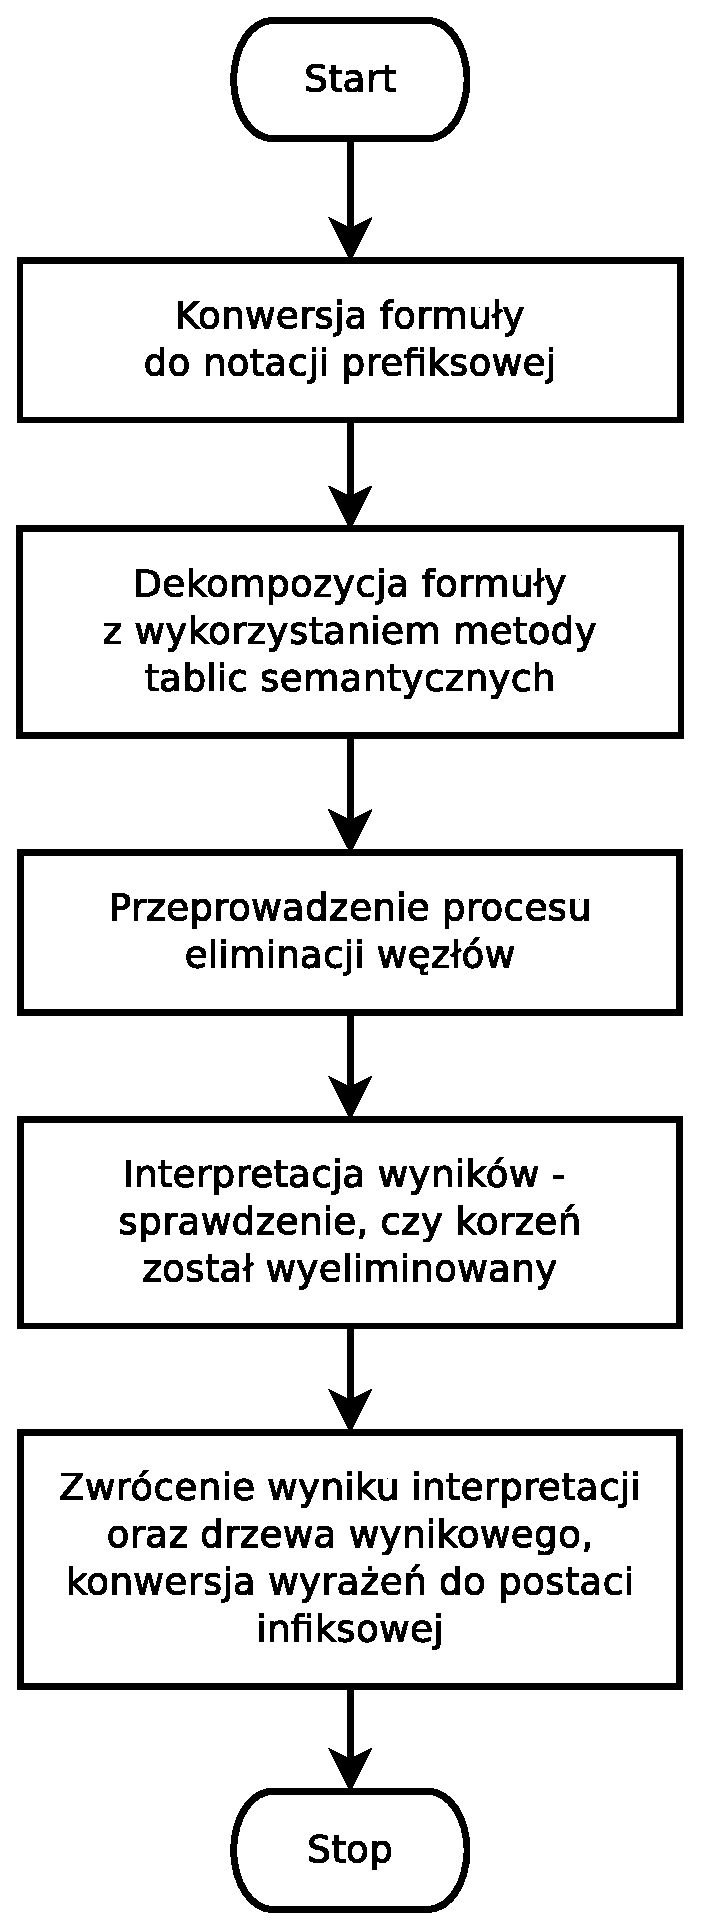
\includegraphics[height=10cm]{main_alg}
\caption{Przebieg głównego algorytmu}
\end{figure}

\subsection{Dekompozycja formuły}

\subsubsection{Reguły dekompozycji}
\label{dekompozycja}

\begin{longtable}{|c|c|}
\hline
\textbf{Postać dekompozycji} & \textbf{Nazwa}\\
\hline
\Tree [.{$p \wedge q$} [.{$p$ \\ $q$} ] ] &  Koniunkcja\\
\hline
\Tree[.{$p \vee q$} {$p$} {$q$} ] &  Alternatywa\\
\hline
\Tree[.{$p \Rightarrow q$} {$\neg p$} {$q$} ] &  Implikacja\\
\hline
\Tree[.{$p \Leftrightarrow q$} {$p$ \\ $q$} {$\neg p$ \\ $\neg q$} ] &  Ekwiwalencja\\
\hline
\Tree [.{$\neg(p \wedge q)$} {$\neg p$} {$\neg q$} ] &  Negacja koniunkcji\\
\hline
\Tree [.{$\neg(p \vee q)$} [.{$\neg p$ \\ $\neg q$} ] ] &  Negacja alternatywy\\
\hline
\Tree [.{$\neg(p \Rightarrow q)$} [.{$p$ \\ $\neg q$} ] ] &  Negacja implikacji\\
\hline
\Tree[.{$\neg(p \Leftrightarrow q)$} {$p$ \\ $\neg q$} {$\neg p$ \\ $q$} ] &  Negacja ekwiwalencji\\
\hline
\Tree [.{$\neg \neg p$} [.{$p$} ] ] &  Negacja negacji\\
\hline
\Tree [.{$\neg X p$} [.{$X \neg P$} ] ] &  Negacja operatora \textit{Next}\\
\hline
\Tree[.{$F p$} {$p$} {$X F p$} ] &  Operator \textit{Finally}\\
\hline
\Tree[.{$\neg F p$} [.{$\neg p$ \\ $\neg X F p$} ] ] & Negacja operatora \textit{Finally}\\
\hline
\Tree[.{$p U q$} {$q$} [.{$p$ \\ $X ( p U q)$} ] ] &  Operator \textit{Until}\\
\hline
\Tree [.{$\neg (p U q) $} [.{$\neg q$ \\ $\neg p \vee \neg X (p U q)$} ] ] &  Negacja operatora \textit{Until}\\
\hline
\Tree[.{$G p$} {$p$} {$X G p$} ] &  Operator \textit{Globally}\\
\hline
\end{longtable}

\subsubsection{Algorytm metody tablic semantycznych}
\label{tableau}
Metoda tablic semantycznych opiera się o budowanie drzewa (w zasadzie grafu skierowanego, który może zostać uproszczony do drzewa, co wyjaśniono w punkcie \ref{Implementacja}) poprzez dekomponowanie kolejnych podwyrażeń składających się na wejściową formułę logiczną zgodnie z zasadami przytoczonymi w \ref{dekompozycja}. W trakcie dekompozycji kolejne powstające podformuły (a także węzły drzewa) oznaczane są jako sprawdzone, w celu uniknięcia ich kilkukrotnego przetwarzania. Odrzucenie ich nie jest możliwie, ze względu na konieczność odwoływania się do węzłów poprzedzających w niektórych krokach algorytmu.
\linebreak
Algorytm metody tablic semantycznych przebiega następująco:
\begin{enumerate}
	\item Tworzenie korzenia drzewa zawierającego formułę wejściową (lub jej zaprzeczenie)
	\item Dekompozycja następnego w kolejności wyrażenia logicznego. Kolejność dekomponowania wyrażeń znajdujących się w węzłach drzewa jest dowolna, jednak ze względu efektywność algorytmu najlepiej przyjąć następujący porządek:
	\begin{itemize}
	\item[1.] Dekomponowanie wyrażeń niepowodujących rozgałęziania
	\item[2.] Dekomponowanie wyrażeń powodujących rozgałęzianie oraz tworzących dwa pod-wyrażenia w węzłach potomnych
	\item[3.] Dekomponowanie wyrażeń powodujących rozgałęzianie oraz tworzących jedno wyrażenie w węzłach potomnych
	\end{itemize}
	\item W przypadku węzła, który zawiera wyrażenia z operatorem \textit{Next} - rozszerzenie drzewa, przez przyłączenie potomka zawierającego wyrażenia nieatomiczne, z usuniętym zewnętrznym operatorem \textit{Next}, lub w przypadku gdy takie wyrażenie już występowało w nadrzędnym węźle, utworzenie ścieżki do tego węzła (jest to połączenie cykliczne)
	\item Punkt 2 i 3 algorytmu powtarza się, dopóki w drzewie znajdują się niesprawdzone, nieelementarne wyrażenia
	\item Eliminacja węzłów - węzeł oznacza się jako usunięty, jeśli:
	\begin{itemize}
	\item[1.] Zawiera on dwie osobne formuły, które są wyrażeniem atomicznym i jego zaprzeczeniem
	\item[2.] Wszyscy potomkowie danego węzła zostali usunięci
	\item[3.] Jeśli węzeł zawiera wyrażenia postaci $F p$ lub $q U p$ i jeśli nie istnieje w drzewie ścieżka prowadząca do węzła zawierającego formułę $p$ 
	\end{itemize}
	\item Interpretacja wyników - jeżeli korzeń drzewa został usunięty, to formuła jest niespełnialna (w przypadku, gdy w korzeniu zostało podane jej zaprzeczenie jest spełnialna)
\end{enumerate}

\subsection{Implementacja}
\label{Implementacja}

\begin{figure}[!htb]
\centering
\includegraphics[width=13cm]{classDiagram}
\caption{Diagram klas składowych}
\end{figure}

W kolejnych podpunktach przedstawiony został uproszczony (niezawierający szczegółów implementacyjnych nieistotnych w kontekście zasady działania) opis implementacji algorytmu metody tablic semantycznych.

\subsubsection{Reprezentacja formuły logicznej}
Za reprezentację pojedynczej formuły logicznej odpowiada klasa \textit{StringFormula}. Operuje ona na wyrażeniach zapisanych w postaci infiksowej (w notacji polskiej), co znacznie ułatwia ich parsowanie i dekompozycję. Formuła przechowywana jest w postaci tablicy tokenów (\textit{tokenArray}, typ \textit{token} jest typem wyliczeniowym stanowiącym semantyczną definicję tokena) oraz w postaci odpowiadających im symboli (\textit{symbolArray}). Klasa \textit{StringFormula} implementuje wszystkie metody, które w algorytmie operują na jednostkowych formułach logicznych:
\begin{itemize}
	\item Wykonującej właściwą dekompozycję formuły logicznej (\textit{decompose()}) zwracającej typ wykonanej dekompozycji reprezentowanej przez typ wyliczeniowy \textit{decomposeType})
	\item Określającej typ następnej dekompozycji (\textit{getType()})
	\item Określającej, czy formuła składa się tylko ze zmiennej logicznej (\textit{isPreposition()}) lub jej zaprzeczenia (\textit{isPrepositionNegation()})
	\item Określającej, czy formuła jest pusta (\textit{isEmpty()})
	\item Zwracającej podformułę logiczną (\textit{needsSatisfaction()}), której istnienie jest wymagane do spełnienia formuły (patrz \ref{tableau}, punkt 5)
\end{itemize}


\subsubsection{Reprezentacja węzła drzewa}
\label{node}
Pojedynczy węzeł drzewa dekompozycji jest reprezentowany przez klasę \textit{FormulaNode}. Jej podstawowym atrybutem jest tablica przechowywanych formuł logicznych (\textit{formulas}) oraz odpowiadająca im tablica, określająca, czy dana formuła została już przetworzona (\textit{isChecked}). Poza tymi elementami, obiekt tej klasy przechowuje również informację o wyeliminowaniu węzła, który reprezentuje (\textit{eliminated}, oraz powiązane z tym atrybutem metody \textit{isEliminated()} i \textit{setEliminated()}). Ostatnim kluczowym atrybutem jest iterator (\textit{feedbackPath}) wskazujący na węzeł zawierający formułę po usunięciu skrajnego operatora temporalnego \textit{Next} (opisano w \ref{tableau}). W przypadku obiektu klasy \textit{tree} pochodzącego z biblioteki \textit{tree.hh} iterator stanowi najprostszy sposób na odwołania się do danego elementu drzewa. Przechowywanie referencji do węzła (w tej specyficznej postaci) pozwala na zredukowanie podstawowej struktury danych do postaci drzewa (zamiast grafu skierowanego). Oczywiście zabieg ten posiada dalsze implikacje (opisane w \ref{tree}).

\begin{figure}[!htb]
\centering
\includegraphics[width=9cm]{Diagram2}
\caption{Zastąpienie ścieżki cyklicznej w grafie (a) dodatkową zmienną w węźle, przechowującą referencję (b)}
\end{figure}

W skład klasy \textit{FormulaNode} wchodzą również wszystkie inne metody konieczne do wykonania algorytmu:
\begin{itemize}
	\item Przyłączenie formuły logicznej do węzła (\textit{appendFormula()})
	\item Sprawdzenie, czy węzeł jest pusty (\textit{isEmpty()})
	\item Określenie, jakie formuły muszą zostać spełnione, aby węzeł nie został odrzucony (\textit{toSatisfy()}, opisano w \ref{tableau})
	\item Sprawdzenie, czy węzeł zawiera daną formułę (\textit{contains()})
	\item Wykonanie dekompozycji kolejnej formuły, zgodnie z heurystyką przedstawioną w \ref{tableau}. Dodatkowo w celu zwiększania wydajności obliczeniowej po powstaniu każdego nowego węzła rozpatrywana jest możliwość jego eliminacji, co pozwala na uniknięcie dalszej dekompozycji węzłów niemających wpływu na całościowy wynik działania
\end{itemize}

\subsection{Reprezentacja drzewa dekompozycji}
\label{tree}
Ostatnią kluczową klasą składową jest klasa \textit{TruthTree}, agregująca obydwie przedstawione wcześniej podklasy, reprezentująca drzewo dekompozycji formuły. Jest to \textit{wrapper} klasy drzewa zdefiniowanej w bibliotece \textit{tree.hh}. Poza głównym drzewem dekompozycji (\textit{mainTree}), w klasie przechowywana jest informacja o korzeniu drzewa (w postaci iteratora). W skład metod klasy wchodzą istotne metody pomocnicze, tzn. \textit{existsPath} oraz \textit{findFormula}. Pierwsza z nich sprawdza istnienie ścieżki pomiędzy dwoma węzłami wchodzącymi w skład głównego drzewa, a więc umożliwia rozstrzygnięcie problemu eliminacji węzła w przypadku wystąpienia operatorów temporalnych \textit{Finally} i \textit{Until}. W implementacji metody wzięto pod uwagę możliwość wystąpienia ścieżki cyklicznej (reprezentowanej w sposób omówiony w \ref{node}), która może być skutkiem obecności operatora temporalnego \textit{Next}. Metoda \textit{findFormula} pozwala na określenie, czy w całym drzewie wystąpiła dana formuła logiczna i w którym węźle się ona znajduje. Podstawowymi metodami, wywoływanymi przez użytkownika końcowego są:
\begin{itemize}
	\item Przeprowadzenie całego procesu dekompozycji wejściowej formuły (\textit{decomposeAll()})
	\item Przeprowadzenie jednego kroku dekompozycji (\textit{decomposeStep()})
	\item Przeprowadzenie procesu eliminacji węzłów (\textit{eliminateNodes()}) - jego wykonanie po zakończeniu wykonania algorytmu jest konieczne, pomimo wspomnianej (\ref{node}) eliminacji częściowej
	\item Określenie spełnialności formuły (\textit{getResult()})
\end{itemize}

\end{document}
